% Template for Elsevier CRC journal article
% version 1.2 dated 09 May 2011

% This file (c) 2009-2011 Elsevier Ltd.  Modifications may be freely made,
% provided the edited file is saved under a different name

% This file contains modifications for Procedia Computer Science

% Changes since version 1.1
% - added "procedia" option compliant with ecrc.sty version 1.2a
%   (makes the layout approximately the same as the Word CRC template)
% - added example for generating copyright line in abstract

%-----------------------------------------------------------------------------------

%% This template uses the elsarticle.cls document class and the extension package ecrc.sty
%% For full documentation on usage of elsarticle.cls, consult the documentation "elsdoc.pdf"
%% Further resources available at http://www.elsevier.com/latex

%-----------------------------------------------------------------------------------

%%%%%%%%%%%%%%%%%%%%%%%%%%%%%%%%%%%%%%%%%%%%%%%%%%%%%%%%%%%%%%
%%%%%%%%%%%%%%%%%%%%%%%%%%%%%%%%%%%%%%%%%%%%%%%%%%%%%%%%%%%%%%
%%                                                          %%
%% Important note on usage                                  %%
%% -----------------------                                  %%
%% This file should normally be compiled with PDFLaTeX      %%
%% Using standard LaTeX should work but may produce clashes %%
%%                                                          %%
%%%%%%%%%%%%%%%%%%%%%%%%%%%%%%%%%%%%%%%%%%%%%%%%%%%%%%%%%%%%%%
%%%%%%%%%%%%%%%%%%%%%%%%%%%%%%%%%%%%%%%%%%%%%%%%%%%%%%%%%%%%%%

%% The '3p' and 'times' class options of elsarticle are used for Elsevier CRC
%% The 'procedia' option causes ecrc to approximate to the Word template
\documentclass[3p,times,procedia]{elsarticle}
\flushbottom

%% The `ecrc' package must be called to make the CRC functionality available
\usepackage{ecrc}
\usepackage[bookmarks=false]{hyperref}
    \hypersetup{colorlinks,
      linkcolor=blue,
      citecolor=blue,
      urlcolor=blue}
%\usepackage{amsmath}


%% The ecrc package defines commands needed for running heads and logos.
%% For running heads, you can set the journal name, the volume, the starting page and the authors


%% set the starting page if not 1
\firstpage{1}


%% Give the author list to appear in the running head
%% Example \runauth{C.V. Radhakrishnan et al.}
\runauth{Comănac Dragoș-Mihail}



%% Hereafter the template follows `elsarticle'.
%% For more details see the existing template files elsarticle-template-harv.tex and elsarticle-template-num.tex.

%% Elsevier CRC generally uses a numbered reference style
%% For this, the conventions of elsarticle-template-num.tex should be followed (included below)
%% If using BibTeX, use the style file elsarticle-num.bst

%% End of ecrc-specific commands
%%%%%%%%%%%%%%%%%%%%%%%%%%%%%%%%%%%%%%%%%%%%%%%%%%%%%%%%%%%%%%%%%%%%%%%%%%

%% The amssymb package provides various useful mathematical symbols

\usepackage{amssymb}
%% The amsthm package provides extended theorem environments
\usepackage{amsthm}
\usepackage{amsmath}
\usepackage{multirow}
\usepackage{comment}

%% The lineno packages adds line numbers. Start line numbering with
%% \begin{linenumbers}, end it with \end{linenumbers}. Or switch it on
%% for the whole article with \linenumbers after \end{frontmatter}.
%% \usepackage{lineno}

%% natbib.sty is loaded by default. However, natbib options can be
%% provided with \biboptions{...} command. Following options are
%% valid:

%%   round  -  round parentheses are used (default)
%%   square -  square brackets are used   [option]
%%   curly  -  curly braces are used      {option}
%%   angle  -  angle brackets are used    <option>
%%   semicolon  -  multiple citations separated by semi-colon
%%   colon  - same as semicolon, an earlier confusion
%%   comma  -  separated by comma
%%   numbers-  selects numerical citations
%%   super  -  numerical citations as superscripts
%%   sort   -  sorts multiple citations according to order in ref. list
%%   sort&compress   -  like sort, but also compresses numerical citations
%%   compress - compresses without sorting
%%
%% \biboptions{authoryear}

% \biboptions{}

% if you have landscape tables
\usepackage[figuresright]{rotating}
%\usepackage{harvard}
% put your own definitions here:x
%   \newcommand{\cZ}{\cal{Z}}
%   \newtheorem{def}{Definition}[section]
%   ...

% add words to TeX's hyphenation exception list
%\hyphenation{author another created financial paper re-commend-ed Post-Script}

% declarations for front matter

%\pagenumbering{gobble}

\begin{document}
\begin{frontmatter}

%% Title, authors and addresses

%% use the tnoteref command within \title for footnotes;
%% use the tnotetext command for the associated footnote;
%% use the fnref command within \author or \address for footnotes;
%% use the fntext command for the associated footnote;
%% use the corref command within \author for corresponding author footnotes;
%% use the cortext command for the associated footnote;
%% use the ead command for the email address,
%% and the form \ead[url] for the home page:
%%
%% \title{Title\tnoteref{label1}}
%% \tnotetext[label1]{}
%% \author{Name\corref{cor1}\fnref{label2}}
%% \ead{email address}
%% \ead[url]{home page}
%% \fntext[label2]{}
%% \cortext[cor1]{}
%% \address{Address\fnref{label3}}
%% \fntext[label3]{}

\dochead{\huge{Advanced Methods in Data Analysis}}%
%% Use \dochead if there is an article header, e.g. \dochead{Short communication}
%% \dochead can also be used to include a conference title, if directed by the editors
%% e.g. \dochead{17th International Conference on Dynamical Processes in Excited States of Solids}


\title{\textbf{You Only Look Once: Arhitectural discussion}}

%% use optional labels to link authors explicitly to addresses:
%% \author[label1,label2]{<author name>}
%% \address[label1]{<address>}
%% \address[label2]{<address>}



\author{Comănac Dragoș-Mihail} 

\address{dragos.comanac@stud.ubbcluj.ro}

\begin{abstract}
%% Text of abstract
%Context
Billions of people that suffer from some form of visual impairment, out of which a significant part is legally blind. Also, a basic human need is mobility, but there aren't enough traditional mobility solutions for all visually impaired persons, such as assistance dogs, thus, for most legally blind people this need can't be easily satisfied. A more scalable solution would be a digital one, which involves computer vision. %This is possible because recent advances in hardware enable complex computations on mobile devices, and computer vision has emerged as a key field of artificial intelligence because it aims to replicate the human visual cortex. 

%This kind of solution could be easily distributed to the millions of legally blind people because a mobile phone is much cheaper and more common than an assistance dog, for instance.

%Objective
Therefore, the main purpose of this paper is to provide a form of mobile assistive technology, based on object detection for visually impaired persons.

%The idea is that the object detector takes as input live images from the mobile device's camera and outputs bounding boxes that describe surrounding objects. Finally, this information is converted to sound and played using the mobile device's speakers. In this way, visually impaired persons can gather valuable information about the environment and travel through it.

%Method

Our object detector is implemented along the lines of You Only Look Once. We train on a subset of Open Images V4 dataset composed of bus, car, and license plate, a single convolutional neural network. Also, we have developed an Android mobile application that uses this object detector in order to visualize the bounding box predictions. The key feature of the application is the accessible live object detection, in which the predictions are converted to sound and played using the mobile device speakers. %This is the proof of concept for the assistive technology that uses computer vision, on low-budget hardware, such as a mobile phone.

%Results

We obtain a mean average precision of 70.03\%, and for the bus class, we obtain an average precision of 90.01\%, for the car class 64.04\% and for the license plate 56.68\%, with a speed of around 5 FPS on a mobile device. 

%We have also trained a model on the COCO dataset that achieves around 0.4\% mAP on the test dataset. The result is modest, but the object detection system was built around the Open Images V4 dataset, and we tried to obtain a model that is as small as possible in order to consume few resources. 


\end{abstract}

\begin{keyword}

%% keywords here, in the form: keyword \sep keyword
Object detection \sep Deep learning \sep YOLO
%% MSC codes here, in the form: \MSC code \sep code
%% or \MSC[2008] code \sep code (2000 is the default)


\end{keyword}
\end{frontmatter}



%%
%% Start line numbering here if you want
%%
% \linenumbers

%% main text

%\enlargethispage{-7mm}

\section{Introduction}\label{introduction}

You Only Look Once (YOLO) \cite{yolo} is a widely used method for performing object detection. It is a one-stage object detection method well suited for performance in real-time. Here, the object detection is modeled as a regression problem, as opposed to the more complex and long pipeline of two-stage object detectors. The real-time performance is essentially achieved by greatly reducing the inference time using end-to-end learning. The network can benefit from this by directly predicting the class probabilities and bounding boxes from the image.
        
Beside speed, the relatively easy to implement architecture is another reason for its popularity, or the fact that usually the neural networks that implement this architecture can be quite small, therefore they are suitable for deployment on devices with limited computing power. 

The importance of this subject comes from the need for fast and precise methods such as YOLO for finding objects in visual data such as images and videos. Some fields in which this method can be successfully implemented (among others) include the automotive industry with use cases such as autonomous driving, traffic monitoring, or parking management, and logistics with use cases such as inventory management. 

Also, the authors of YOLO do not provide a detailed explanation of their implementation, leaving out only the key details, and their implementation is written using their C library implemented from scratch, by them, thus the code is not necessarily trivial to understand. Given these circumstances, we hope that this paper could serve as a guide for a step by step implementation of an YOLO object detection pipeline. 

Given the potential of this subject, the aim of this paper is to study the YOLO method and the reasons behind its success. In what follows, we integrate the topic in the general field in Section \ref{placement} and we give a description of the method in Section \ref{method}. Also, we present other object detection methods in Section \ref{related_work} and we compare YOLO with them in Section \ref{comparison}.


%Given the potential of deep neural networks in solving the problem of object detection, the purpose of this paper is to study the popular neural network architecture proposed in You Only Look Once (YOLO) \cite{yolo}. 
\section{Placement in the broader field} \label{placement}

Computer vision is a scientific field that deals with the extraction of meaningful information from visual data such as images or videos. As a consequence, over time, computer vision has emerged as a key field in the domain of artificial intelligence because it intends to replicate the functions of the human visual cortex. This is possible due to the continuous development of optical hardware, which nowadays can exceed the capabilities of the human eye, but probably more important are the huge quantities of data that are available to more and more people.

There are various methods that can be used in the field of computer vision, such as hand crafted features, but in this context of big data, the most relevant methods are related to machine learning, and more recently to deep learning which is better suited to visual data. Through supervised learning, deeper and deeper neural network models are now able to learn the complex patterns found in large amounts of data, thus they are a good fit for solving computer vision problems.

One such problem is object detection, which consists of locating and classifying objects in an image. This problem is relevant in many domains such as automotive, logistics or even assistive technologies. Also, it has more potential than simple classification, because the objects are localized and this forces the learning algorithm to look for the very specific patterns that describe the objects, as opposed to classification where other patterns might be learned if the data distribution is unbalanced.

Broadly speaking, in the context of neural networks, the object detection problem mainly branches out in two-stage object detection which traditionally was slow, but accurate and one-stage object detection which initially was less accurate and fast, but recently they became better and better, even surpassing the performance of two-stage object detectors.

The first modern object detectors split the object detection problem into several tasks, which composed a pipeline that is often difficult to train, hence they are collectively named two-stage object detectors. The first steps taken into this direction were made by region-based object detectors such as R-CNN \cite{rcnn} and the later faster versions. Essentially, the bounding boxes are generated through selective search, after which a convolutional neural network is used to extract feature maps that are then classified.

One-stage object detectors achieve real-time speed with good accuracy because their detection pipeline consists only of one convolutional neural network that processes the image and directly outputs the predictions. This approach used to have low accuracy due to the lack of large amounts of data, but recent advances have made the one-stage detectors rival the two-stage detectors in terms of accuracy, without losing speed. YOLO falls into this one-stage class of object detectors, hence it's success in achieving good performance, with little resources.
\section{Method description} \label{method}

In this section we describe the arhitectural details of the neural network behind the YOLO method. 

\subsection{General architecture overview}

As we have previously mentioned, the key element in one-stage methods is the fact that there is only one convolutional neural network that learns end-to-end to predict the bounding boxes from the entire image. It is a common practice to split the neural network architecture in three parts, as we have depicted in Fig. \ref{architecture}. Each section of this general architecture are important and deserves comprehensive studies on their own.

\begin{figure}[!h]
  \centering
  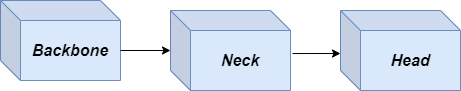
\includegraphics[scale=0.5]{images/objdet_structure.png}
  \caption{General neural network architecture for one-stage object detectors}
      \label{architecture}
\end{figure} 

The role of the backbone is to extract feature maps from the original image, that describe for instance various shapes which can help in determining the location and class of the possible objects. Depending on the precision and speed requirements the specific design of the backbone can vary from small networks, used for speed, or large networks, used for better precision. The actual design can be custom, but if there is not enough data to accommodate the required size of the network, a common practice is to use transfer learning. 

The idea is to use an already existent network architecture that is trained on a large amount of diverse data. Usually, a network used for classification is used by replacing the last layers with the neck and head architecture specific for the given problem. In this way, the extracted knowledge from the larger source dataset is stored in the network and it can be reused on the target dataset. How many layers are cut from the image classifier neural network depends on how similar are the target and source dataset. Also, regarding training, the first step is to train the whole network with the backbone frozen in order to not break the knowledge stored in its weights and the second step is to train the whole network with the backbone unfrozen, but with a low learning rate, in order to better fit the target dataset. For example a ResNet like architecture \cite{resnet} can be used if high precision is needed, or a MobileNet like architecture \cite{mobilenetv1, mobilenetv2} is suitable if speed is of the essence.

The neck is an optional component and its main role is to be an intermediary between the backbone and the head, such that it further refines the features from the backbone in order to provide more information for the head. An example for the neck architecture is the Feature Pyramid Network \cite{fpn}. The idea is that there are several feature maps extracted from the backbone that are provided to the head, in order to let the network to "see" at several resolutions.

If the other two components are not necessarily that specific to object detection, the head is responsible for taking the output of the neck (or directly from the backbone if the neck does not exist), optionally refine them furthermore, and finally converting them to the desired representation. This is the part where YOLO method contributes the most. Basically, it describes how the head should convert a feature maps into a representation from which bounding boxes can be extracted.

\subsection{YOLO head}

The main idea behind YOLO is that in order to detect multiple objects, at various locations, the image is split in a grid in which each cell is responsible for detecting objects that appear inside it. In fact, this is the representation of the ground truth labels.

\subsubsection{Ground truth definition}

The ground truth is represented as a $C \times C \times B \times (5+N)$ tensor. For each cell in the $C \times C$ grid, there are B anchor boxes associated. Each anchor box has the following parameters: $b_x$ and $b_y$ represent the center of the box and they are both relative to the cell responsible for predicting the object, meaning that they are divided to the size of the cell, $b_w$ and $b_h$ represent the width and height, c is the probability that the anchor predicts an object and $c_1, c_2, c_3, ... c_n$ represent the $N$ class probabilities, hence the $5+N$ term. The actual choice for the size of the grid, the number of anchors or the number of classes is problem specific. They are important because they determine the maximum number of positives in an image. The problem of defining positives in object detection is also an important concern.

When choosing anchors there are mainly two approaches. Either they are set by hand, or they are computed through a clustering algorithm over the whole dataset. The authors for example use K-Means, with one cluster per anchor, in order to better fit the patterns of the bounding boxes in the dataset. 

In the original version of the method, each cell is responsible for predicting only one bounding box, meaning that the idea of anchors is not used. As it's the case with many algorithms, anchors are only an optimization. Technically speaking, in ideal conditions, with enough data, it is enough to have one predictor per cell in order to regress any object. But as it it's often the case, there is not enough data, therefore, anchors were introduced for simplicity in the idea that it is good to split a complex problem in multiple simpler problems. The idea is that there are multiple predictors per cell that can learn various objects shapes. In this way, one predictor can specialize in tall objects and another in wide objects for instance. This also helps if there are multiple overlapped objects corresponding to one cell. 

In order to create the ground truth for an image, the bounding box labels must contain the center of the object, its width and its height. The way this information is expressed can vary, but it is not important as long as the center, width and height can be computed. The next step is to find the cell in which the center of the object falls into. That cell will be responsible for detecting the object. Then the anchor that is the closest to the object in terms of shape must be chosen. This is done using Intersection Over Union (IOU). 

\subsubsection{Interpretation of the raw output}

Regarding the network design, the final layer has the same structure as the ground truths. One way this can be implemented is with a 1x1 (pointwise) convolution. In order to do this, the layer before the pointwise convolution should output a feature map with a spatial size of $C \times C$. The number of channels does not matter because it is controlled by the pointwise convolution which has $B * (5 + N)$ kernels in order to output a feature map of size $C \times C \times (B * (5+N))$ which can be further reshaped to a tensor of shape $C \times C \times B \times (5+N)$ in order to match the shape of the ground truth.

The height, width and the coordinates of the object center are computed using the following formulas:
\begin{equation}
\begin{split}
    & bbox_x = \sigma(z_x) + c_x \\
    & bbox_y = \sigma(z_y) + c_y \\
    & bbox_w = a_w \cdot e^{z_w} \\ 
    & bbox_h = a_h \cdot e^{z_h} \\
    & bbox_obj = \sigma(z_{obj})
\end{split}
\label{conversion_formulas}
\end{equation}

The network predicts the raw values $z_x, z_y, z_w, z_h$. The upper left corner of the predicting cell is given by $c_x, c_y$ and are needed because the coordinates of the center are represented in the grid coordinate system. The width and height are relative to the predicting anchor, hence $a_w, a_h$ are used in computing the width and height of the object. Another value is predicted, that predicts the objectness $z_{obj}$ of the bounding box, meaning that it represents the probability that there is a bounding box predicted by the anchors. Also, the softmax can be used in order to get the class probabilities, which are further multiplied with the objectness score. In order to compute the loss it is enough to leave $bbox_x$ and $bbox_y$ as they are, but they are relative to the predicting grid cell and in order to get the actual bounding box relative to the image, $bbox_x$ and $bbox_y$ need to be multiplied with the size of the grid cell in order to get them in the coordindate system of the image.

As it is the case with most object detectors, YOLO can benefit from using Non-maximum Suppression. A common problem in object detection are the overlapping bounding boxes that actually predict the same object. The role of Non-maximum Suppression is to prune away extra bounding boxes. The first step is to order descending the bounding boxes by their objectness scores. The boxes are parsed one by one, and they are kept if the IOU with any bounding box of the same class previously kept is below a certain threshold. Hence only, the bounding box with the highest score will be kept in a certain region. As the object detectors become denser and denser, this operation becomes a very relevant one. There are also resarch interest in finding object detection methods that do not need this filtering due to its computational cost.


\subsection{Methodologies based on YOLO}

The success of the YOLO method is given by the robustness it has shown through time. Over the years, several methodologies have been proposed that use YOLO as the key element. Each brings different optimizations over the original method, but the main aspects are still relevant. For example, the second version of YOLO \cite{yolov2} mainly introduces the notion of anchors and a novel multi-scale training method in order to have good predictions across images of various scales. The third version of YOLO \cite{yolov3} represents mostly a bundle of small improvements. 

YOLO gained such a success that the original author has stopped its research in the field of artificial intelligence due to the fact that his work could be used to do harm, in modern warfare for example. In spite of this, the research into this method did not stop, because other people have developed several newer optimizations over the original algorithm. Also, this might be due to the fact that YOLO is very relevant in the industry of embedded computing, being a top choice for systems that have low resources and need to perform the task of object detection.

For instance, object detectors such as YOLOv7 \cite{yolov7} and YOLOX \cite{yolox} use the YOLO method in modern methodologies. The newer training techniques and optimizations resulted in competitive object detectors which achieve state of the art results. In YOLOX the authors propose an anchor free solution, and in YOLOv7 the authors continued an existing trend, that of finding methods that improve the performance without increasing the number of parameters, hence the speed loss is minimized.

The fact that there is still an ongoing research interest into this method is another argument for its success and robustness.
\section{Related work} \label{related_work}

In order to have a better understanding of YOLO, we aim in section to describe other well known methods.

\subsection{Single Shot MultiBox Detector}

Single shot MultiBox Detector (SSD) \cite{ssd} is another example of an object detection system that achieves real-time performance, encapsulating all operations in a single deep neural network. Like YOLO, this helps SSD to outperform in terms of speed previous approaches that use multiple stages in detection such as R-CNN. 
     
The network architecture is similar to the one of YOLO, or to the single shot object detectors architectures in general. As such, the network is composed mainly of two parts, and optionally the neck. The first one is the same and consists of what is called the base network, which is a truncated version of an image classifier, where the classification layers are removed, that is used to extract features. On top of the base network, several structures specific to object detection are added.
        
The key features of SSD are the multi-scale feature maps, convolutional predictors, and default boxes. 
        
        \begin{figure}[h]
          \centering
          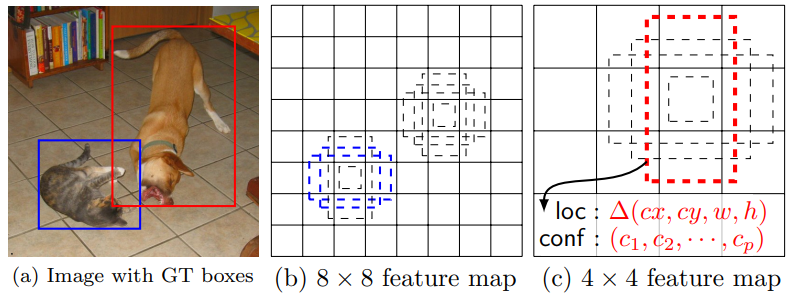
\includegraphics[scale=0.6]{images/ssd.png}
          \caption{Visualization of the feature maps used in SSD \cite{ssd}}
          \label{ssdImg}
        \end{figure}
        
The main difference between this method and YOLO is that to the base network, there are appended several convolutional layers that decrease progressively in size the feature map from the base network. This way predictions are made for each newly added layer, therefore, the predictions are made at various scales, as it is depicted in Fig. \ref{ssdImg}. 
        
Each cell in each feature map has associated K default bounding boxes, whose positions are relative to their cell. Then for each box several kernels of size $3 \times 3 \times P$, where $M \times N$ is the size of the feature map and P is the number of channels, are used to predict C class probabilities and 4 offsets to the respective box. This means that each box uses $(C+4)\cdot K$ filters, therefore the size of the predictions is $(C+4)  \times  K \times M \times N$.
        
During training, the outputs need to be assigned to their corresponding ground truths. Then the loss function and backpropagation are applied end-to-end. Furthermore, the set of default boxes and scales is chosen, and hard negative mining and data augmentation strategies are used.
        
For matching the outputs, each ground truth box is associated with the default box with the highest Jaccard overlap. The novel approach here is that the default boxes are also matched with any ground truth box with a Jaccard overlap higher than a threshold. This allows predictions with high scores for multiple overlapping default boxes.
        
%The loss is a weighted sum between confidence loss and localization loss.
        
Another crucial part is choosing scales and aspect ratios for the default boxes. Each feature map has a specific scale, distributed evenly between two values. The aspect ratios are chosen from a predefined set. The width and height are computed using the scale and the aspect ratio. The center is chosen based on the feature map cell size.
        
The matching steps produce more negatives than positives. This introduces an imbalance, and to fix this, the negatives are filtered by their confidence loss so that a ratio of three to one is kept between the negatives and positives.
        
%Also, data augmentation is used. During training for each image either a patch is randomly sampled, a path is sampled so that the minimum Jaccard overlap with the objects is higher than a threshold, or the original image is used. After this, the image is resized and flipped with a probability of 0.5, and some photometric distortions are applied.

\subsection{Region based convolutional neural networks}

This type of method falls into the category of two-stage object detectors. Traditionally, there was a clean separation in terms of performance between this type of object detectors and the one stage class of object detectors, but with time, both types of methods became better in what they lacked by bringing several optimizations over the original architecture. Two stage methods gained speed and one stage methods gained accuracy for example.

In Fig. \ref{rcnnImg} we can observe why this method is a two-stage type of method. Basically, the first stage is to extract from the input image a lot of region proposals or region of interests. Ideally, these region proposals contain objects of interest and will represent the final bounding box. Here we can observe the fundamental difference between two-stage methods and YOLO, or one-stage methods in general. In one-stage methods, the bounding boxes are obtained through regression, while in two-stage methods, they are extracted beforehand. It is important to note that R-CNN is agnostic to the way region proposals are extracted from the input image, as the authors mention. One way the region proposals can be extracted is by selective search, which is the method adopted originally by the authors and it does not involve any learning. Another way is to obtain them through a what is called a region proposal network that is a fully convolutional network capable of predicting both bounding boxes and objectness scores.

\begin{figure}[h]
  \centering
  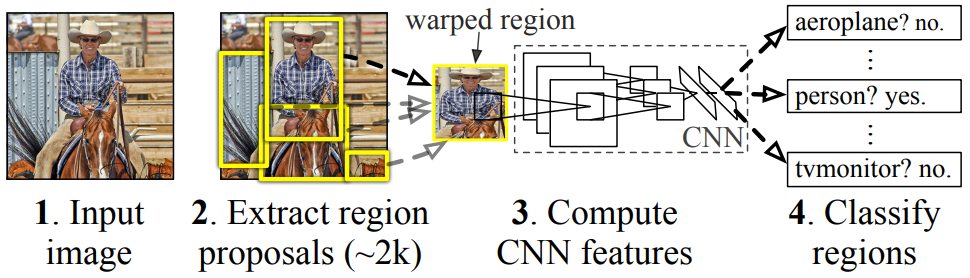
\includegraphics[scale=0.4]{images/rcnn.png}
  \caption{Two stage pipeline used in R-CNN \cite{rcnn}}
  \label{rcnnImg}
\end{figure}

Region proposal is a complex domain and it deserves focused research on it's own. The idea is that it is crucial for two-stage method to have good proposals in order to achieve high performance. This could be seen as a downside compared to it's counterparts, the one-stage methods, because it adds a layer of extra complexity. Also, the density of region proposals is crucial, this also being related to a more general problem in object detection, that of defining positives. Thus, if there aren't enough proposals, the network performance will be limited in the sense that it will not be able to find all objects and the recall can be affected.

The second step is to take the region proposals and classify them. Optionally, the region proposals can be further refined before being classified. The classification can be done in several ways such as with artificial neural networks, convolutional neural networks or support vector machines.

The final predictions are composed from the bounding boxes given by the region proposals and the classification scores resulted from the second stage.

This method as it is can achieve good performance in terms of precision but it lacks speed. This is mostly due to the fact that many region proposals are actually overlapping, thus there are a lot of extra computations that have a negative impact on the speed. This was further optimized in Fast R-CNN \cite{fastRcnn} by introducing a convolutional neural network as a preliminary step before selective search in order to then compute region proposals on the processed feature maps using region of interest pooling. In this way, the feature extraction becomes a shared computation. Another optimization is proposed in Faster R-CNN \cite{fasterRcnn} and it consists of replacing selective search with a region proposal network, that can learn to predict a set of object proposals, together with their objectness scores directly from the extracted feature maps, resulted by passing the input image through a convolutional neural network. These optimizations greatly reduce the inference time, and maintain good performance, but the method still lacks behind one-stage methods such as YOLO in terms of speed.



\section{Comparison with other methods in terms of performance} \label{comparison}

In this section we aim to give a quantitative comparison on standard object detection datasets of the YOLO method and the methods described in Section \ref{related_work}. 

To measure an object detection system performance usually frames per second (FPS) and mean average precision (mAP) are the most relevant measures. FPS simply means the number of images, or frames, an algorithm can process in a single second.

%In order to see how accurate the model is, mAP is used. To compute mAP, first, the predictions are sorted descending by their confidence score. Then, the predictions are parsed one by one, and at each step, the precision and recall are computed, taking into consideration only the parsed prediction up until that point. For the recall, we consider all positives, including those that were not parsed. If we would plot these values, with the recall on the horizontal axis and the precision on the vertical axis, we would get what is called the precision-recall curve. Average precision is defined as the area under the precision-recall curve and mAP is defined as the mean of the average precisions for each class.

Over time, this mAP measure became the standard when it comes to measuring the quality of an object detection system.

The first standard dataset in object detection research was The Pascal Visual Object Classes \cite{pascal-voc} and it started out as an object detection challenge. Basically, the researchers that came up with new ideas in this domain had to use this dataset in order to compare their methods with the existing literature. Additionally, in order for the comparison to be fair, the authors of the dataset also published the code for computing mAP.

In Fig. \ref{pascal} we detail the mAP values for some object detectors described early. We can see that the original YOLO methodology lags behind other object detectors, but the second one, which introduces anchors, surpasses them all.


\def \scalevar {0.6}

\begin{figure}[!h]
  \centering
  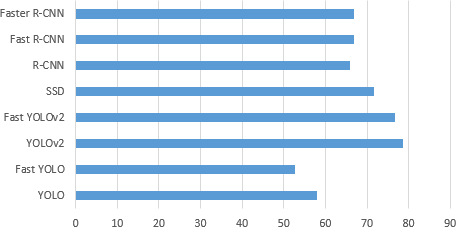
\includegraphics[scale=\scalevar]{images/pascal.png}
  \caption{Performances over the Pascal VOC dataset in terms of mAP}
  \label{pascal}
\end{figure}

As the technology advanced, researchers were able to train on larger and larger datasets, thus the Microsoft Common Objects in Context (COCO) dataset \cite{coco} became the new standard that new object detection methodologies use in order to be relevant in the field. Also, the authors provide an evaluation server which allows a better comparison between object detectors. The idea is that the labels for the test set are not publicly available, only the images can be downloaded. Therefore, the researchers that propose new object detection methods, have to upload on the evaluation server their results on the test set, and get back a detailed mAP evaluation for various thresholds and for small, medium and large objects.

We also perform a comparison on the newer standard COCO dataset in Fig. \ref{coco}. Here we can observe that YOLO had a constant positive evolution through time on this dataset.

\begin{figure}[!h]
  \centering
  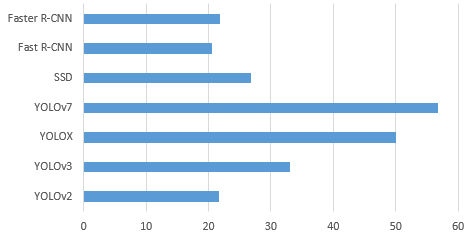
\includegraphics[scale=\scalevar]{images/coco.png}
  \caption{Performances over the COCO dataset in terms of mAP}
  \label{coco}
\end{figure}


Also, another crucial aspect is the speed. In Fig. \ref{fps} we detail the reported speeds in FPS. This measure is relevant in practical applications, because usually, the hardware is a pretty rigid constraint, and as such the neural network that runs on the hardware must meet the some speed constraints in order to run as expected from the point of view of the application. For example, R-CNN like methods are better suited for applications where real time speed is not crucial, and the others are built specifically for real time speeds.

\begin{figure}[!h]
  \centering
  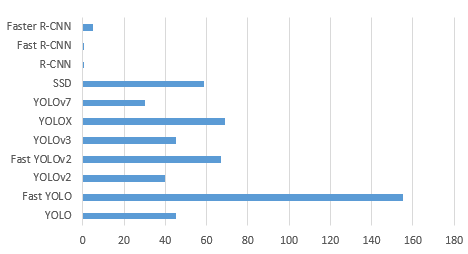
\includegraphics[scale=\scalevar]{images/speed.png}
  \caption{Performances in terms of frames per second}
  \label{fps}
\end{figure}





%Regarding performance on the Pascal VOC 2007 dataset, SSD achieves 74.3\% mAP and 59 FPS, surpassing the first version of YOLO in terms of speed and accuracy balance.
        
%On the Microsoft COCO and in the context in which YOLOv4 was tested, described in \cite{yolov4}, SSD achieves 43 FPS with 25.1\% mAP. This shows that YOLO surpasses SSD in terms of prediction quality, with minimal time costs.


%According to \cite{yolo}, in terms of performance on the Pascal VOC 2007 dataset \cite{pascal-voc-2007}, the first version of YOLO achieves 63.4\% mAP and 45 frames per second (FPS), and the faster version has 52.7\% mAP and 155 FPS. For comparison, Faster R-CNN \cite{fasterRcnn} achieves 73.2\% mAP but 7 FPS, which is accurate but very slow, and the Deformable parts model \cite{30hzDPM} achieves 100 FPS but it has 16\% mAP, or a slower variant achieves 26.1\% mAP at 30 FPS. Therefore YOLO strikes a good balance between speed and accuracy.
    
%Newer versions of YOLO bring some incremental improvements. Also, the Microsoft COCO dataset \cite{coco} is another relevant dataset for comparing object detection systems. On this dataset, YOLOv4 \cite{yolov4} achieves 43.9\% mAP at 31 FPS, or a smaller variant achieves 38 FPS, with 41.2\% mAP.


\section{Conclusions}
    In conclusion, YOLO is an important milestone for the object detection domain. The main innovations are that it managed to create a single viable and successful convolutional neural network architecture that is able to learn end to end to predict the bounding boxes from the raw data, as opposed to two-stage methods such as R-CNN. This is possible due to the change of mindset, because in YOLO the problem of object detection is modeled as a regression.
    
    All of these discussed factors have sustained the quality in time, making it a robust method for performing object detection. This is proven by the constant ongoing research into this method and the competitive results resulted from this research. 
    
    Looking towards the future, we believe that the method is generic and versatile enough that it can be adapted to the newest advances in deep learning in general, as it was the case until the time of writing this paper. We also argue that this method is a good candidate for various practical applications in our modern society, given the low computational cost and relatively easy to understand and implement architecture.
    
        



\footnotesize{

\bibliographystyle{elsarticle-harv}
\bibliography{biblio}

} 

\end{document}

%%
%% End of file `Sample Paper.tex'.
